\documentclass[../lecture-notes.tex]{subfiles}

\begin{document}

\subsection{Finite Field Extensions}

\subsubsection{General Definition}

Previously, our discussion resolved around the finite field $\mathbb{F}_p$ for a prime $p$. However, many protocols
need more than just a prime field. For example, elliptic curve pairings and certain STARK constructions require
extending $\mathbb{F}_p$ to, in a sense, the analogous of complex numbers. 

From school and, possibly, university, you might remember how complex numbers $\mathbb{C}$ are constructed. You take two real numbers, say, $x,y \in \mathbb{R}$, introduce a new
symbol $i$ satisfying $i^2 = -1$, and define the complex number as $z = x + iy$. In certain cases, one might encounter a bit more rigorous and abstract definition of complex numbers as
the set of pairs $(x,y) \in \mathbb{R}^2$ where addition in naturally defined as $(x_1,y_1)+(x_2,y_2)=(x_1+x_2,y_1+y_2)$, and the multiplication is:
\begin{equation}
    (x_1,y_1) \cdot (x_2,y_2) = (x_1x_2-y_1y_2,x_1y_2+x_2y_1)\footnote{Notice that $(x_1+iy_1)(x_2+iy_2) = x_1x_2+iy_2x_1+iy_1x_2+i^2y_1y_2 = (x_1x_2-y_1y_2) + (x_1y_2+x_2y_1)i$.}.
\end{equation}

In spite of what interpretation you have seen, the complex number is just a tuple of two real numbers that satisfy a bit different rules of multiplication (since addition is typically defined in the same way). What is even more important to us, is that $\mathbb{C}$ is our first example of the so-called \textbf{field extension} of $\mathbb{R}$.

Formally, definition of the field extension is very straightforward:
\begin{definition}
    Let $\mathbb{F}$ be a field and $\mathbb{K}$ be another field. We say that $\mathbb{K}$ is an \textbf{extension} of $\mathbb{F}$ if $\mathbb{F} \subset \mathbb{K}$ and we denote it as $\mathbb{K}/\mathbb{F}$.
\end{definition}

Despite just a simplicity of the definition, the field extensions are a very powerful tool in mathematics. But first, let us consider a few non-trivial examples of field extensions.

\begin{example}
    Denote by $\mathbb{Q}(\sqrt{2}) = \{x + y\sqrt{2}: x,y \in \mathbb{Q}\}$. This is a field extension of $\mathbb{Q}$. It is obvious that $\mathbb{Q} \subset \mathbb{Q}(\sqrt{2})$, but why is $\mathbb{Q}(\sqrt{2})$ a field? Addition and multiplication operations are obviously closed:
    \begin{equation}
        \begin{aligned}
            (x_1+y_1\sqrt{2}) + (x_2+y_2\sqrt{2}) = (x_1+x_2) + (y_1+y_2)\sqrt{2},\\
            (x_1+y_1\sqrt{2}) \cdot (x_2+y_2\sqrt{2}) = (x_1x_2+2y_1y_2) + (x_1y_2+x_2y_1)\sqrt{2}.
        \end{aligned}
    \end{equation}
    But what about the inverse element? Well, here is the trick:
    \begin{equation}
        \frac{1}{x+y\sqrt{2}} = \frac{x-y\sqrt{2}}{(x+y\sqrt{2})(x-y\sqrt{2})} = \frac{x-y\sqrt{2}}{x^2-2y^2} = \frac{x}{x^2-2y^2} - \frac{y}{x^2-2y^2}\sqrt{2} \in \mathbb{Q}(\sqrt{2}).
    \end{equation}
\end{example}

\begin{example}
    Consider $\mathbb{Q}(\sqrt{2}, i) = \{a+bi: a,b \in \mathbb{Q}(\sqrt{2})\}$ where $i^2=-1$. This is a field extension of $\mathbb{Q}(\sqrt{2})$ and, consequently, of $\mathbb{Q}$. The representation of the element is:
    \begin{equation}
        (a+b\sqrt{2}) + (c+d\sqrt{2})i = a + b\sqrt{2} + ci + d\sqrt{2}i
    \end{equation}

    Showing that this is a field is a bit more tedious, but still straightforward. Suppose we take $\alpha+\beta i \in \mathbb{Q}(\sqrt{2}, i)$ with $\alpha,\beta \in \mathbb{Q}(\sqrt{2})$. Then:
    \begin{equation}
        \frac{1}{\alpha+\beta i} = \frac{\alpha-\beta i}{\alpha^2+\beta^2} = \frac{\alpha}{\alpha^2+\beta^2} - \frac{\beta}{\alpha^2+\beta^2}i
    \end{equation}

    Since $\mathbb{Q}(\sqrt{2})$ is a field, both $\frac{\alpha}{\alpha^2+\beta^2}$ and $\frac{\beta}{\alpha^2+\beta^2}$ are in $\mathbb{Q}(\sqrt{2})$, and, consequently, $\mathbb{Q}(\sqrt{2}, i)$ is a field as well.
\end{example}

\begin{remark}
    Notice that basically, $\mathbb{Q}(\sqrt{2}, i)$ is just a linear combination of $\{1,\sqrt{2},i,\sqrt{2}i\}$. This has a very important implication: $\mathbb{Q}(\sqrt{2}, i)$ is a four-dimensional vector space over $\mathbb{Q}$, where elements $\{1,\sqrt{2},i,\sqrt{2}i\}$ naturally form \textbf{basis}. We are not going to use it implicitly, but this observation might make further discussion a bit more intuitive.
\end{remark}

\begin{remark}
    One might have defined $\mathbb{Q}(\sqrt{2}, i) = \{x+\sqrt{2}y: x,y \in \mathbb{Q}(i)\}$ instead. Indeed, $\mathbb{Q}(\sqrt{2})(i) = \mathbb{Q}(i)(\sqrt{2}) = \mathbb{Q}(\sqrt{2}, i)$.
\end{remark}

\subsubsection{Polynomial Quotient Ring}

Now, we present a more general way to construct field extensions. Notice that when constructing $\mathbb{C}$, we used the magical element $i$ that satisfies $i^2=-1$. But here is another way how to think of it.

Consider the set of polynomials $\mathbb{R}[x]$, then I pick $p(x):=x^2+1 \in \mathbb{R}[x]$ and ask you to find roots of $p(x)$. Of course, you would claim ``hey, this equation has no solutions over $\mathbb{R}$'' and that is totally true. That is why mathematicians introduced a new element $i$ that we formally called the root of $x^2+1$. Note however, that $i$ is not a number in the traditional sense, but rather a fictional symbol that we artifically introduced to satisfy the equation.

Now, could we have picked another polynomial, say, $q(x) = x^2+4$? Sure! As long as its roots cannot be found in $\mathbb{R}$, we are good to go.

\begin{example}
    Suppose $\beta$ is the root of $q(x):=x^2+4$. Then we could have defined complex numbers as a set of $x+y\beta$ for $x,y \in \mathbb{R}$. In this case, multiplication, for example, would be defined a bit differently than in the case of $\mathbb{C}$:
    \begin{equation}
        (x_1+y_1\beta) \cdot (x_2+y_2\beta) = (x_1x_2-4y_1y_2) + (x_1y_2+x_2y_1)\beta.
    \end{equation}
\end{example}

We shifted to the polynomial consideration for a reason: now, instead of considering the complex number $\mathbb{C}$ as ``some'' tuple of real numbers $(c_0,c_1)$, now let us view it as a polynomial\footnote{Here, we use $X$ to represent the polynomial variable to avoid confusion with the notation $x+yi$.} $c_0+c_1X$ modulo polynomial $X^2+1$. 

\begin{example}
Indeed, take, for example, $p_1(X) := 1+2X$ and $p_2(X) := 2+3X$. Addition is performed as we are used to:
\begin{equation}
    p_1 + p_2 = (1+2X) + (2+3X) = 3+5X,
\end{equation}
but multiplication is a bit different:
\begin{equation}
    p_1p_2 = (1+2X) \cdot (2+3X) = 2+3X+4X+6X^2 = 6X^2+7X+2.
\end{equation}

Well, and what next? Recall that we are doing arithmetic modulo $X^2+1$ and for that reason, we divide the polynomial by $X^2+1$:
\begin{equation}
    6X^2+7X+2 = 6(X^2+1) + 7X - 4 \implies (6X^2+7X+2) \,\text{mod}\, (X^2+1) = 7X-4,
\end{equation}
meaning that $p_1p_2 = 7X-4$. Oh wow, hold on! Let us come back to our regular complex number representation and multiply $(1+2i)(2+3i)$. We get $2+3i+4i+6i^2=-4+7i$. That is exactly the same result if we change $X$ to $i$ above! In fact, what we have observed is the fact that our polynomial quotient ring $\mathbb{R}[X]/(X^2+1)$ is isomorphic to $\mathbb{C}$.
\end{example}

So, let us generalize this observation to any field $\mathbb{F}$ and any irreducible polynomial $\mu(x) \in \mathbb{F}[x]$.

\begin{theorem}
    Let $\mathbb{F}$ be a field and $\mu(x)$ --- irreducible polynomial over $\mathbb{F}$ (sometimes called a \textbf{reduction polynomial}). Consider a set of polynomials over $\mathbb{F}[x]$ modulo $\mu(x)$, formally denoted as $\mathbb{F}[x]/(\mu(x))$. Then, $\mathbb{F}[x]/(\mu(x))$ is a field.
\end{theorem}

\begin{example}
    As we considered above, let $\mathbb{F}=\mathbb{R}$, $\mu(x)=x^2+1$, then $\mathbb{R}[X]/(X^2+1)$ (a set of polynomials modulo $X^2+1$) is a field.
\end{example}
\begin{example}
    Suppose $\mathbb{F}=\mathbb{Q}$ and $\mu(x) := x^2-2$. Then, $\mathbb{Q}[X]/(X^2-2)$ is a field isomorphic to $\mathbb{Q}(\sqrt{2})$, considered above.
\end{example}
\begin{example}
    Suppose $\mathbb{F}=\mathbb{Q}$ and $\mu(x) := (x^2+1)(x^2-2)=x^4-x^2-2$. Then, $\mathbb{Q}[X]/(x^4-x^2-2)$ is a field isomorphic to $\mathbb{Q}(\sqrt{2},i)$.
\end{example}

\begin{remark}
    Although we have not defined the isomorphism between two rings/fields, it is defined similarly to group isomorphism. Suppose we have fields $(\mathbb{F},+,\times)$ and $(\mathbb{K}, \oplus, \otimes)$. Bijective function $\phi: \mathbb{F} \to \mathbb{K}$ is called an isomorphism if it preserves additive and multiplicative structures, that is for all $a,b \in \mathbb{F}$:
    \begin{equation}
        \begin{aligned}
            \phi(a+b) = \phi(a) \oplus \phi(b),\\
            \phi(a\times b) = \phi(a) \otimes \phi(b).
        \end{aligned}
    \end{equation}
\end{remark}

This theorem (aka definition) corresponds to viewing complex numbers as a polynomial quotient ring $\mathbb{R}[X]/(X^2+1)$. But, we can give a theorem (aka definition) for our classical representation via magical root $i$ of $x^2+1$.

\begin{theorem}
    Let $\mathbb{F}$ be a field and $\mu \in \mathbb{F}[X]$ is an irreducible polynomial of degree $n$ and let $\mathbb{K} := \mathbb{F}[X]/(\mu(X))$. Let $\theta \in \mathbb{K}$ be the root of $\mu$ over $\mathbb{K}$. Then,
    \begin{equation}
        \mathbb{K} = \{c_0+c_1\theta+\cdots+c_{n-1}\theta^{n-1}: c_0,\dots,c_{n-1} \in \mathbb{F}\}
    \end{equation}
\end{theorem}

Although this definition is quite useful, we will mostly rely on the polynomial quotient ring definition. Let us define the \textbf{prime field extension}.

\begin{definition}
    Suppose $p$ is prime and $m \geq 2$. Let $\mu \in \mathbb{F}_p[X]$ be an irreducible polynomial of degree $m$. Then, elements of $\mathbb{F}_{p^m}$ are polynomials in $\mathbb{F}_p^{(\leq m)}[X]$. In other words,
    \begin{equation}
        \mathbb{F}_{p^m} = \{c_0+c_1X+\cdots+c_{m-1}X^{m-1}: c_0,\dots,c_{m-1} \in \mathbb{F}_p\},
    \end{equation}
    where all operations are performed modulo $\mu(X)$.
\end{definition}

Again, let us consider a few examples.

\begin{example}
    Consider the $\mathbb{F}_{2^4}$. Then, there are $16$ elements in this set:
    \begin{equation}
        \begin{aligned}
            &0, 1, X, X+1,\\ &X^2, X^2+1, X^2+X, X^2+X+1,\\
            &X^3, X^3+1, X^3+X, X^3+X+1,\\ &X^3+X^2, X^3+X^2+1, X^3+X^2+X, X^3+X^2+X+1.
        \end{aligned}
    \end{equation}

    One might choose the following reduction polynomial: $\mu(X)=X^4+X+1$ (of degree $4$). Then, operations are performed in the following manner:
    \begin{itemize}
        \item Addition: $(X^3+X^2+1)+(X^2+X+1) = X^3+X$.
        \item Subtraction: $(X^3+X^2+1)-(X^2+X+1) = X^3+X$.
        \item Multiplication: $(X^3+X^2+1)\cdot(X^2+X+1)=X^2+1$ since:
        \begin{equation}
            (X^3+X^2+1)\cdot(X^2+X+1) = X^5+X+1 \; \text{mod} \; (X^4+X+1) = X^2+1
        \end{equation}
        \item Inversion: $(X^3+X^2+1)^{-1}=X^2$ since $(X^3+X^2+1)\cdot X^2 \; \text{mod} \; (X^4+X+1) = 1$.
    \end{itemize}
\end{example}

Now, in the subsequent sections, we would need to extend $\mathbb{F}_p$ at least to $\mathbb{F}_{p^2}$. A convenient choice, similarly to the complex numbers, is to take $\mu(X)=X^2+1$. However, in contrast to $\mathbb{R}$, equation $X^2=-1 \pmod{p}$ might have solutions over certain prime numbers $p$. Thus, we consider proposition below.

\begin{proposition}
    Let $p$ be an odd prime. Then $X^2+1$ is irreducible in $\mathbb{F}_p[X]$ if and only if $p \equiv 3 \pmod{4}$.
\end{proposition}

\begin{corollary}
    $\mathbb{F}_{p^2} = \mathbb{F}_p[u]/(u^2+1)$ is a valid prime field extension for odd primes $p$ satisfying $p \equiv 3 \pmod{4}$. In this case, extended elements are of the form $c_0+c_1u$ where $c_0,c_1 \in \mathbb{F}_p$ and $u^2=-1$.
\end{corollary}

\subsubsection{Multiplicative Group of a Finite Field}\label{section:multiplicative_subgroup}

The non-zero elements of $\mathbb{F}_p$, denoted as $\mathbb{F}_p^{\times}$, form a multiplicative cyclic group. In other words, there exist elements $g \in \mathbb{F}_p^{\times}$, called \textit{generators}, such that
\begin{equation}
    \mathbb{F}_p^{\times} = \{g^k: 0 \leq k \leq p-2\}
\end{equation}

The order of $x \in \mathbb{F}_p^{\times}$ is the smallest positive integer $r$ such that $x^r=1$. It is also not difficult to show that $r \mid (p-1)$.

\begin{definition}
    $\omega \in \mathbb{F}$ is the \textit{primitive root} in the finite field $\mathbb{F}$ if $\langle\omega\rangle = \mathbb{F}^{\times}$.
\end{definition}

\begin{example}
    $\omega=3$ is the primitive root of $\mathbb{F}_7$. Indeed,
    \begin{equation}
        \begin{aligned}
            3^1=3, 3^2=2, 3^3=6, 3^4=4, 3^5=5, 3^6=1.
        \end{aligned}
    \end{equation}

    So clearly $\langle \omega \rangle = 7$.
\end{example}

In STARKs (and in optimizing operations) for DFT (Discrete Fourier Transform) we would need the so-called $n$th primitive roots of unity.

\begin{example}
    For those who studied complex numbers a bit (it is totally OK if you did not, so you might skip this example), recall an equation $\zeta^n=1$ over $\mathbb{C}$. The solutions are $\zeta_k = \cos\left(\frac{2\pi k}{n}\right) + i\sin\left(\frac{2\pi k}{n}\right)$ for $k\in\{0,1,\dots,n-1\}$, so one has exactly $n$ solutions (in contrast to $x^n=1$ over $\mathbb{R}$ where there are at most $2$ solutions\footnote{Think why.}). For any solution $\zeta_k$, it is true that $\zeta_k^n=1$, but if one were to consider the subgroup generated by $\zeta_k$ (that is, $\{1,\zeta_k, \zeta_k^2,\dots\}$), then not neccecerily $\langle \zeta_k \rangle$ would enumerate all the roots of unity $\{\zeta_j\}_{j=0}^{n-1}$. For that reason, we call $\zeta_k$ the $n$th primitive root of unity if $\langle \zeta_k \rangle$ enumerates all roots of unity. One can show that this is the case if and only if $\gcd(k,n)=1$. This is always the case for $k=1$, so commonly mathematicians use $\zeta_n$ to denote an expression $\cos \frac{2\pi}{n} + i\sin\frac{2\pi}{n} = e^{2\pi i/n}$.
\end{example}

Yet, let us give the broader definition, including the finite fields case.

\begin{definition}
    $\omega$ is the $n$th primitive root of unity if $\omega^n=1$ and $\omega^k \neq 1$ for all $1 \leq k < n$.
\end{definition}

Note that such $\omega$ exists if and only if $n \mid (p-1)$. 

\subsubsection{Algebraic Closure}

Consider the following interesting question: suppose we have a field $\mathbb{F}$. Is there an extension $\mathbb{K}/\mathbb{F}$ such that $\mathbb{K}$ contains all roots of any polynomial in $\mathbb{F}[X]$? The answer is yes, and such a field is called the \textbf{algebraic closure} of $\mathbb{F}$, although not always this algebraic closure has a nice form. But first, let us define what it means for field $\mathbb{F}$ to be algebraically closed.

\begin{definition}
    A field $\mathbb{F}$ is called \textbf{algebraically closed} if every non-constant polynomial $p(x) \in \mathbb{F}[X]$ has a root in $\mathbb{F}$.
\end{definition}

\begin{example}
    $\mathbb{R}$ is not algebraically closed since $X^2+1$ has no roots in $\mathbb{R}$. However, $\mathbb{C}$ is algebraically closed, which follows from the fundamental theorem of algebra. Since $\mathbb{C}$ is a field extension of $\mathbb{R}$, it is also an algebraic closure of $\mathbb{R}$. This is commonly denoted as $\overline{\mathbb{R}} = \mathbb{C}$.
\end{example}

\begin{definition}
    A field $\mathbb{K}$ is called an \textbf{algebraic closure} of $\mathbb{F}$ if $\mathbb{K}/\mathbb{F}$ is algebraically closed. This is denoted as $\overline{\mathbb{F}} = \mathbb{K}$.
\end{definition}

Since we are doing cryptography and not mathematics, we are interested in the algebraic closure of $\mathbb{F}_p$. Well, I have two news for you (as always, one is good and one is bad). The good news is that any finite field $\mathbb{F}_{p^m}$ has an algebraic closure. The bad news is that it does not have a form $\mathbb{F}_{p^k}$ for $k>m$ and there are infinitely many elements in it (so in other words, the algebraic closure of a finite field is not finite). This is due to the following theorem.

\begin{theorem}
    No finite field $\mathbb{F}$ is algebraically closed.
\end{theorem}

\textbf{Proof.} Suppose $f_1,f_2,\dots,f_n \in \mathbb{F}$ are all elements of $\mathbb{F}$. Consider the following polynomial:
\begin{equation}
    p(x) = \prod_{i=1}^n (x-f_i)+1 = (x-f_1)(x-f_2)\cdots(x-f_n)+1.
\end{equation}

Clearly, $p(x)$ is a non-constant polynomial and has no roots in $\mathbb{F}$, since for any $f \in \mathbb{F}$, one has $p(f)=1$. $\blacksquare$

But what form does the $\overline{\mathbb{F}}_{p}$ have? Well, it is a union of all $\mathbb{F}_{p^k}$ for $k \geq 1$. This is formally written as:
\begin{equation}
    \overline{\mathbb{F}}_{p} = \bigcup_{k \in \mathbb{N}} \mathbb{F}_{p^k}.
\end{equation} 

\begin{remark}
    But this definition is super counter-intuitive! So here how we usually interpret it. Suppose I tell you that polynomial $q(x)$ has a root in $\overline{\mathbb{F}}_p$. What that means is that there exists some extension $\mathbb{F}_{p^m}$ such that for some $\alpha \in \mathbb{F}_{p^m}$, $q(\alpha)=0$. We do not know how large this $m$ is, but we know that it exists. For that reason, $\overline{\mathbb{F}}_p$ is defined as an infinite union of all possible field extensions.
\end{remark}

\subsection{Elliptic Curves}

\subsubsection{Classical Definition}

Probably, there is no need to explain the importance of elliptic curves. Essentially, the main group being used for cryptographic 
protocols is the group of points on an elliptic curve. If elliptic curve is ``good enough'', then the discrete logarithm problem assumption,
Diffie-Hellman assumption and other core cryptographic assumptions hold. Moreover, this group does not require
a large field size, which is a huge advantage for many cryptographic protocols.

So, let us formally define what an elliptic curve is. Further assume that, when speaking of the finite field $\mathbb{F}_p$, the underlying prime number is greater than $3$.\footnote{Note that, for example, for $\mathbb{F}_{2^n}$ equation of elliptic curve is very different, but usually we do not deal with binary field elements.}. The definition is the following.

\begin{definition}
    Suppose that $\mathbb{K}$ is a field. An \textbf{elliptic curve} $E$ over $\mathbb{K}$ is defined as a set of points $(x,y) \in \mathbb{K}^2$:
    \begin{equation}
        y^2 = x^3+ax+b,
    \end{equation}
    called a \textbf{Short Weierstrass equation}, where $a,b \in \mathbb{K}$ and $4a^3+27b^2 \neq 0$. We denote $E/\mathbb{K}$ to denote the elliptic curve over field $\mathbb{K}$.
\end{definition}

\begin{remark}
    One might wonder why $4a^3+27b^2 \neq 0$. This is due to the fact that the curve $y^2=x^3+ax+b$ might have certain degeneracies and special points, which are not desirable for us. So we require this condition to make $E/\mathbb{K}$ ``good''.
\end{remark}

\begin{definition}
    We say that $P=(x_P,y_P) \in \mathbb{A}^2(\mathbb{K})$ is the \textbf{affine representation} of the point on the elliptic curve $E/\mathbb{K}$ if it satisfies the equation $y_P^2=x_P^3+ax_P+b$.
\end{definition}

\begin{example}
    Consider the curve $E/\mathbb{Q}: y^2=x^3-x+9$. This is an elliptic curve. Consider $P=(0,3), Q=(-1,-3) \in \mathbb{A}^2(\mathbb{Q})$: both are valid affine points on the curve. See \Cref{fig:ec_1}.

    \begin{figure}[H]
        \centering
        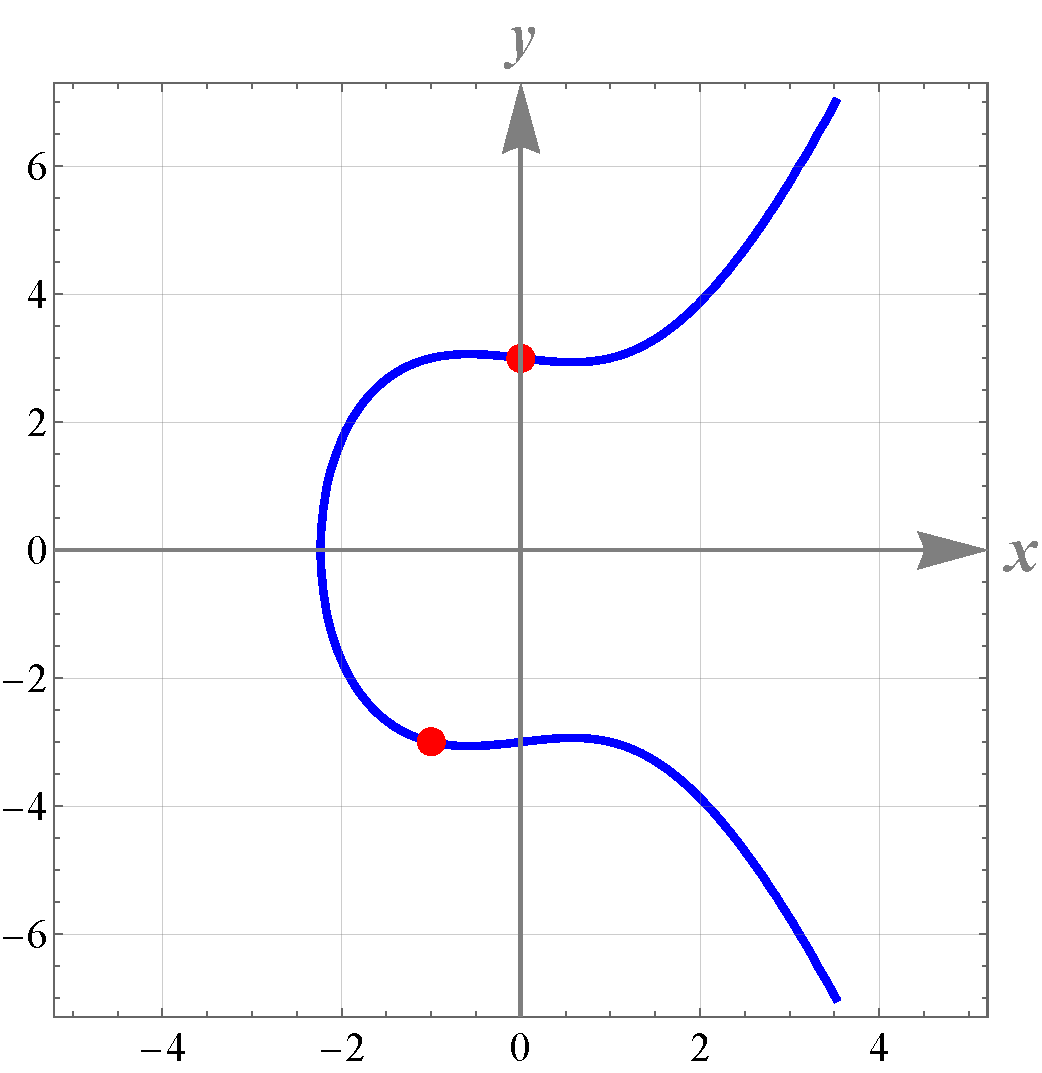
\includegraphics[width=0.5\textwidth]{images/lecture_3/ec_illustration_1.pdf}
        \caption{Elliptic curve $E/\mathbb{Q}: y^2=x^3-x+9$ with points $P=(0,3),Q=(-1,-3)$ depicted on it.}
        \label{fig:ec_1}
    \end{figure}
\end{example}

Typically, our elliptic curve is defined over a finite field $\mathbb{F}_p$, so we are interested in this paricular case. 

\begin{remark}
    Although, in many cases one might encounter the definition where an elliptic curve $E$ is defined over the algebraic closure of $\mathbb{F}_p$, that is $E/\overline{\mathbb{F}}_p$. This is typically important when considering elliptic curve pairings. However, for the sake of simplicity, we will consider elliptic curves over $\mathbb{F}_p$ and corresponding finite extensions $\mathbb{F}_{p^m}$ as of now.
\end{remark}

\begin{remark}
    It is easy to see that if $(x,y) \in E/\mathbb{K}$, then $(x,-y) \in E/\mathbb{K}$. We will use this fact intensively further.
\end{remark}

Now, elliptic curves are useless without any operation defined on top of them. But as will be seen later, it is quite unclear how to define the identity element. For that reason, we introduce a bit different definition of a set of points on the curve.

\begin{definition}
    The set of points on the curve, denoted as $E_{a,b}(\mathbb{K})$, is defined as:
    \begin{equation}
        E_{a,b}(\mathbb{K}) = \{(x,y) \in \mathbb{A}^2(\mathbb{K}): y^2=x^3+ax+b\} \cup \{\mathcal{O}\},
    \end{equation}
    where $\mathcal{O}$ is the so-called \textbf{point at infinity}.
\end{definition}

\begin{remark}
    The difference between $E(\mathbb{K})$ and $E/\mathbb{K}$ is that the former includes the point at infinity, while the latter does not. We also omit the index $a,b$, so instead of $E_{a,b}(\mathbb{K})$ we write simply $E(\mathbb{K})$.
\end{remark}

Now, the reason we introduced the point at infinity $\mathcal{O}$ is because it allows us to define the group binary operation $\oplus$ on the elliptic curve. The operation is sometimes called the \textbf{chord-tangent law}. Let us define it.

\begin{definition}
    Consider the curve $E(\mathbb{F}_{p^m})$. We define $\mathcal{O}$ as the identity element of the group. That is, for all points $P$, we set $P \oplus \mathcal{O} = \mathcal{O} \oplus P = P$. For any other non-identity elements $P=(x_P,y_P),Q=(x_Q,y_Q) \in E(\mathbb{F}_{p^m})$, define the $P\oplus Q = (x_R,y_R)$ as follows:
    \begin{enumerate}
        \item If $x_P\neq x_Q$, use the \textbf{chord method}. Define $\lambda := \frac{y_P-y_Q}{x_P-x_Q}$ --- the slope between $P$ and $Q$. Set the resultant coordinates as:
        \begin{equation}
            x_R := \lambda^2 - x_P - x_Q, \quad y_R := \lambda(x_P-x_R)-y_P.
        \end{equation}
        \item If $x_P=x_Q \wedge y_P=y_Q$ (that is, $P=Q$), use the \textbf{tangent method}. Define the slope of the tangent at $P$ as $\lambda := \frac{3x_P^2+a}{2y_P}$ and set
        \begin{equation}
            x_R := \lambda^2 - 2x_P, \quad y_R := \lambda(x_P-x_R)-y_P.
        \end{equation}
        \item Otherwise, define $P \oplus Q := \mathcal{O}$.
    \end{enumerate}
\end{definition}

The aforementioned definition is illustrated in the Figure below\footnote{Illustration taken from \textit{``Pairing for Beginners''}}.

\begin{figure}[H]
    \centering
    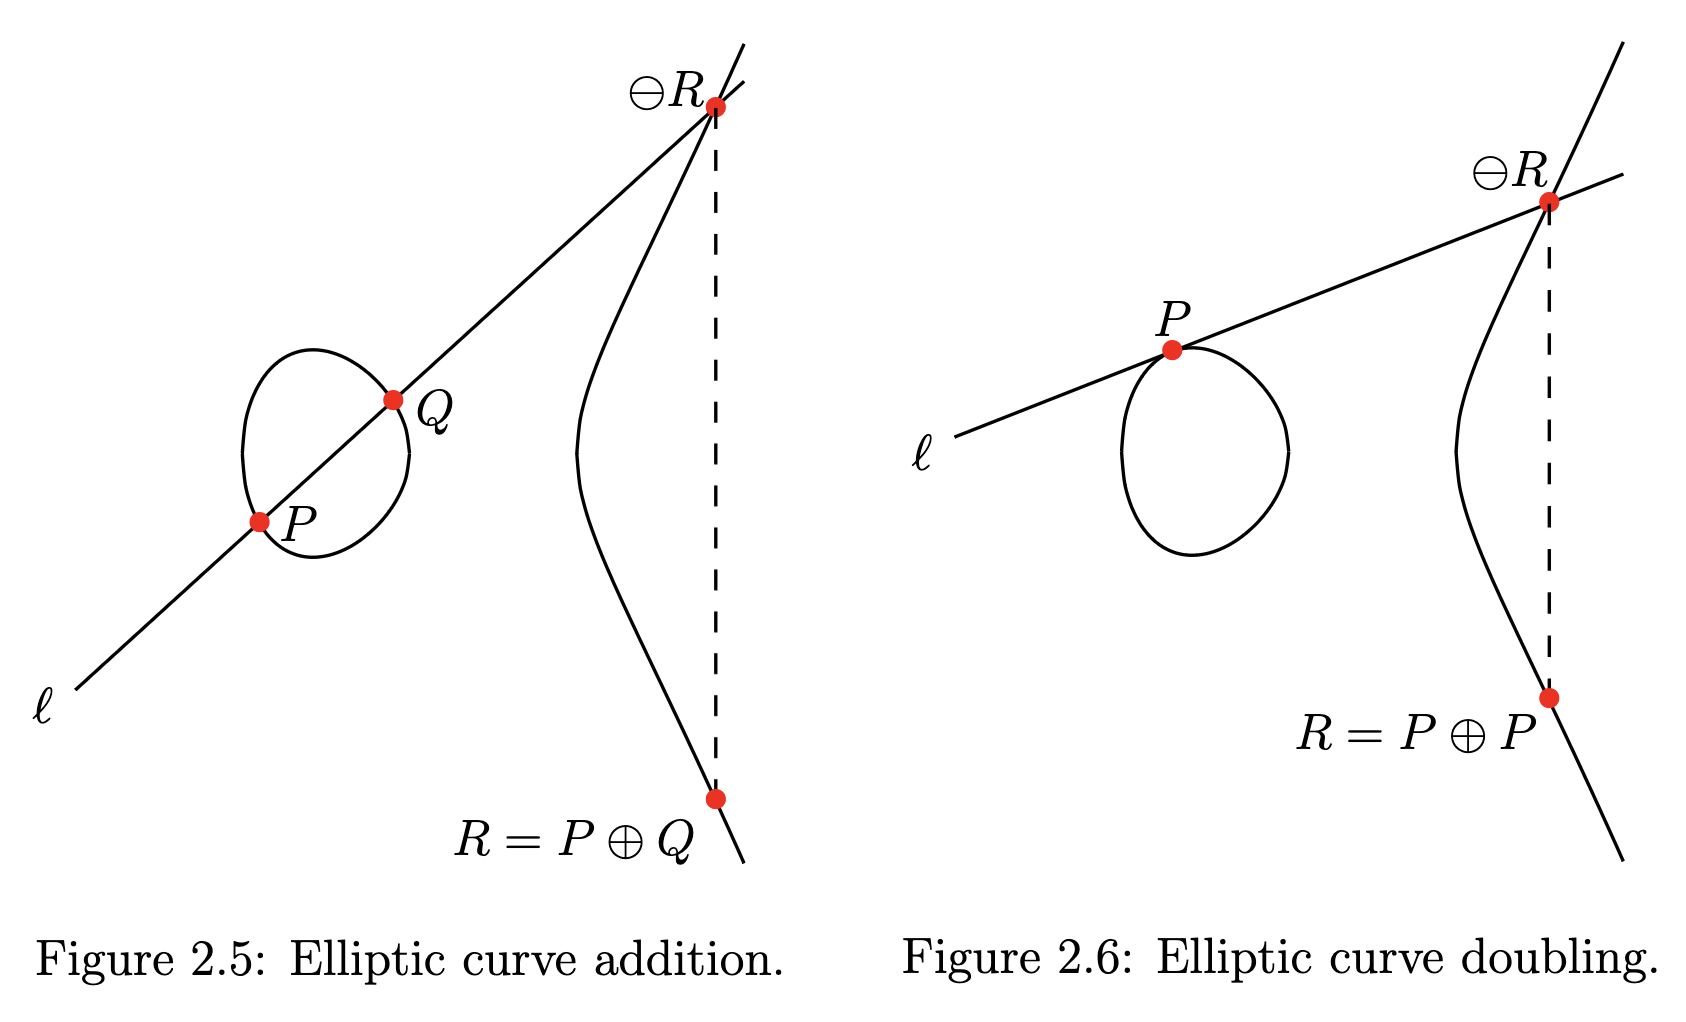
\includegraphics[width=0.7\textwidth]{images/lecture_3/group_law.png}
    \label{fig:group_law}
\end{figure}

\begin{example}
    Consider $E/\mathbb{R}: y^2=x^3-2x$. The points $(-1,-1),(0,0),(2,2)$ are all on $E$ and also on the line $\ell: y=x$. Therefore, $(-1,1) \oplus (0,0) = (2,-2)$ or, similarly, $(2,2) \oplus (-1,-1) = (0,0)$.

    Now, let us compute $[2](-1,-1)$. Calculate the tangent slope as $\lambda := \frac{3\cdot(-1)^2 - 2}{2\cdot(-1)} = -\frac{1}{2}$. Thus, the tangent line has an equation $\ell': y = -\frac{1}{2}x+c$. Substituting $(-1,-1)$ into the equation, we get $c=-\frac{3}{2}$. Therefore, the equation of the tangent line is $y=-\frac{1}{2}x-\frac{3}{2}$. The intersection of the curve and the line is $\left(\frac{9}{4},-\frac{21}{8}\right)$, yielding $[2](-1,-1) = \left(\frac{9}{4},-\frac{21}{8}\right)$.

    The whole illustration is depicted in \Cref{fig:ec_2}.

    \begin{figure}[H]
        \centering
        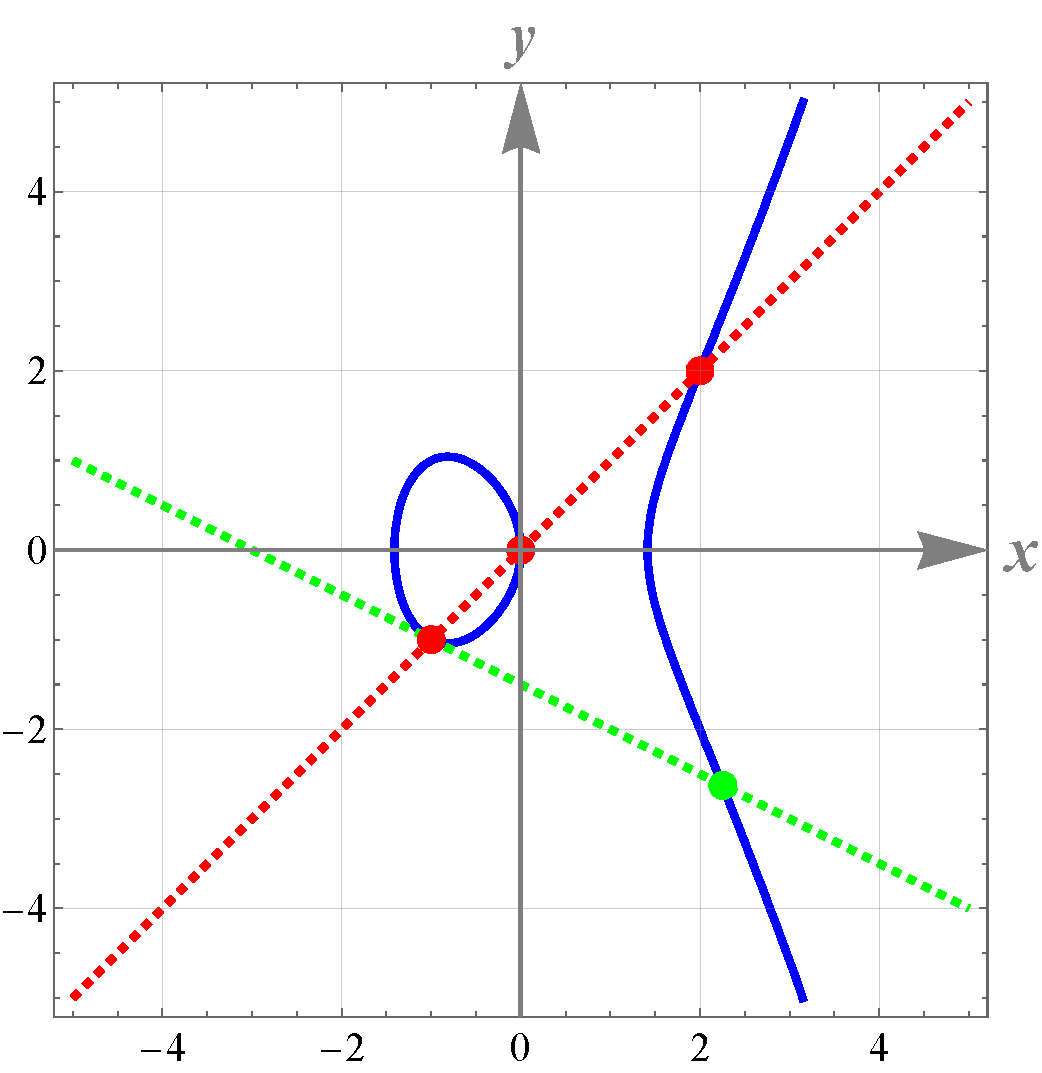
\includegraphics[width=0.4\textwidth]{images/lecture_3/ec_illustration_2.pdf}
        \caption{Illustration of the group law on the elliptic curve $E/\mathbb{R}: y^2=x^3-2x$. In \textcolor{red}{red} we marked points lying on the line $\ell: y=x$. In \textcolor{red}{dashed red}, we marked the line $\ell$, while in \textcolor{green}{dashed green} --- the tangent line $\ell'$ at $(-1,-1)$, which is used to calculate $[2](-1,1)$.}
        \label{fig:ec_2}
    \end{figure}
\end{example}

\begin{theorem}
    $(E(\mathbb{F}_{p^m}),\oplus)$ forms an abelian group.
\end{theorem}

\textbf{Proof Sketch.} The identity element is $\mathcal{O}$. Every point $\mathcal{O} \neq P=(x_P,y_P) \in E(\mathbb{F}_{p^m})$ has an additive inverse: indeed, $\ominus P := (x_P,-y_P)$. Finally, a bit of algebra might show that the operation is associative. It is also clearly commutative: even geometrically it is evident, that the result of $P\oplus Q$ does not depend on the order of $P$ and $Q$ (``drawing a line between $P$ and $Q$'' and ``drawing a line between $Q$ and $P$'' are equivalent statements). $\blacksquare$

Now, let us talk a bit about the group order. The group order is the number of elements in the group. For elliptic curves, the group order is typically denoted as $r$ or $n$, but we are going to use $r$. Also, the following theorem is quite important.

\begin{theorem}
    Define $r := |E(\mathbb{F}_{p^m})|$. Then, $r = p^m + 1 - t$ for some integer $|t| \leq 2\sqrt{p^m}$. A bit more intuitive explanation: the number of points on the curve is close to $p^m+1$. This theorem is commonly called the \textbf{Hasse's theorem on elliptic curves}, and the value $t$ is called the \textbf{trace of Frobenius}.
\end{theorem}

\begin{remark}
    In fact, $r=|E(\mathbb{F}_{p^m})|$ can be computed in $O(\log(p^m))$, so the number of points can be computed efficiently even for fairly large primes $p$.
\end{remark}

Finally, let us define the scalar multiplication operation. 

\begin{definition}
    Let $P \in E(\mathbb{F}_{p^m})$ and $\alpha \in \mathbb{Z}_r$. Define the scalar multiplication $[\alpha]P$ as:
    \begin{equation}
        [\alpha]P = \underbrace{P \oplus P \oplus \cdots \oplus P}_{\alpha \text{ times}}.
    \end{equation}
\end{definition}

\textbf{Question.} Why do we restrict $\alpha$ to $\mathbb{Z}_r$ and not to $\mathbb{Z}$?

\subsubsection{Discrete Logarithm Problem on Elliptic Curves}
Finally, as defined in the previous section, the \textbf{discrete logarithm} problem on the elliptic curve is the following: typically, $E(\mathbb{F}_p)$ is cyclic, meaning there exist some point $G \in E(\mathbb{F}_p)$, called the \textbf{generator}, such that $\langle G \rangle = E(\mathbb{F}_p)$. Given $P \in E(\mathbb{F}_p)$, the problem consists in finding such a scalar $\alpha \in \mathbb{Z}_r$ such that $[\alpha]G = P$. 

Now, if the curve is ``good'', then the discrete logarithm problem is hard. In fact, the best-known algorithms have a complexity $O(\sqrt{r})$. However, there are certain cases when the discrete log problem is much easier.
\begin{enumerate}
    \item If $r$ is composite, and all its prime factors are less than some bound $r_{\max}$, then the discrete log problem can be solved in $O(\sqrt{r_{\max}})$. For this very reason, typically $r$ is prime.
    \item If $|E(\mathbb{F}_p)|=p$, then the discrete logarithm can be solved in polynomial time. These curves are called \textbf{anomalous curves}.
    \item Suppose that there is some small integer $\tau>0$ such that $r \mid (p^{\tau}-1)$. The discrete log in that case reduces to the discrete log in the finite field $\mathbb{F}_{p^{\tau}}$, which is typically not hard for small enough $\tau$.
\end{enumerate}

\subsection{Exercises}
\subsubsection*{Warmup (Oleksandr in search of perfect field extension)}

\textbf{Exercise 1.} Oleksandr decided to build $\mathbb{F}_{49}$ as $\mathbb{F}_7[i]/(i^2+1)$. Compute $(3+i)(4+i)$. 

\begin{enumerate}[a)]
    \item $6+i$.
    \item $6$.
    \item $4+i$.
    \item $4$.
    \item $2+4i$.
\end{enumerate}

\textbf{Exercise 2.} Oleksandr came up with yet another extension $\mathbb{F}_{p^2} = \mathbb{F}_p[i]/(i^2+2)$. He asked interns to calculate $2/i$. Based on five answers given below, help Oleksandr to find the correct one.
\begin{enumerate}[a)]
    \item $1$.
    \item $p-2$.
    \item $(p-3)i$.
    \item $(p-1)i$.
    \item $p-1$.
\end{enumerate}

\textbf{Exercise 3*.} After endless tries, Oleksandr has finally found the perfect field extension: $\mathbb{F}_{p^2} := \mathbb{F}_p[v] / (v^2+v+1)$. However, Oleksandr became very frustrated since not for any $p$ this would be a valid field extension. For which of the following values $p$ such construction would \textbf{not} be a valid field extension? Use the fact that equation $\omega^3=1$ over $\mathbb{F}_p$ has non-trivial solutions (meaning, two others except for $\omega=1$) if $p \equiv 1 \pmod{3}$. You can assume that listed numbers are primes.
\begin{enumerate}[a)]
    \item $8431$.
    \item $9173$.
    \item $9419$.
    \item $6947$.
\end{enumerate}

\begin{tcolorbox}[colback=blue!5!white,fonttitle=\bfseries,colframe=blue!80!white,title=Exercises 4-9. Tower of Extensions]
    \textit{You are given the passage explaining the topic of tower of extensions. The text has gaps that you need to fill in with the correct statement among the provided choices.}
    \vspace{10px}
    
    This question demonstrates the concept of the so-called \textbf{tower of extensions}. Suppose we want to build an extension field $\mathbb{F}_{p^4}$. Of course, we can find some irreducible polynomial $p(X)$ of degree $4$ over $\mathbb{F}_p$ and build $\mathbb{F}_{p^4}$ as $\mathbb{F}_p[X]/(p(X))$. However, this method is very inconvenient since implementing the full $4$-degree polynomial arithmetic is inconvenient. Moreover, if we were to implement arithmetic over, say, $\mathbb{F}_{p^{24}}$, that would make the matters worse. For this reason, we will build $\mathbb{F}_{p^4}$ as $\mathbb{F}_{p^2}[j]/(q(j))$ where $q(j)$ is an irreducible polynomial of degree $2$ over $\mathbb{F}_{p^2}$, which itself is represented as $\mathbb{F}_p[i]/(r(i))$ for some suitable irreducible quadratic polynomial $r(i)$. This way, we can first implement $\mathbb{F}_{p^2}$, then $\mathbb{F}_{p^4}$, relying on the implementation of $\mathbb{F}_{p^2}$ and so on.
    \vspace{5px}

    For illustration purposes, let us pick $p:=5$. As noted above, we want to build $\mathbb{F}_{5^2}$ first. A valid way to represent $\mathbb{F}_{5^2}$ would be to set $\mathbb{F}_{5^2} := \boxed{\textcolor{blue}{\textbf{4}}}$. Given this representation, the zero of a linear polynomial $f(x) = ix - (i+3)$, defined over $\mathbb{F}_{5^2}$, is $\boxed{\textcolor{blue}{\textbf{5}}}$.
    \vspace{5px}

    Now, assume that we represent $\mathbb{F}_{5^4}$ as $\mathbb{F}_{5^2}[j]/(j^2-\xi)$ for $\xi = i+1$. Given such representation, the value of $j^4$ is $\boxed{\textcolor{blue}{\textbf{6}}}$. Finally, given $c_0+c_1j \in \mathbb{F}_{5^4}$ we call $c_0 \in \mathbb{F}_{5^2}$ a \textbf{real part}, while $c_1 \in \mathbb{F}_{5^2}$ an \textbf{imaginary part}. For example, the imaginary part of number $j^3+2i^2\xi$ is $\boxed{\textcolor{blue}{\textbf{7}}}$, while the real part of $(a_0+a_1j)b_1j$ is $\boxed{\textcolor{blue}{\textbf{8}}}$. Similarly to complex numbers, it motivates us to define the number's \textbf{conjugate}: for $z = c_0+c_1j$, define the conjugate as $\overline{z} := c_0-c_1j$. The expression $z\overline{z}$ is then $\boxed{\textcolor{blue}{\textbf{9}}}$.
\end{tcolorbox}

\begin{center}
    \begin{tabular}{p{5cm}p{5cm}p{5cm}}
        % Exercise 3
        \textbf{Exercise 4.}
        \begin{enumerate}[a)]
            \item $\mathbb{F}_5[i]/(i^2+1)$
            \item $\mathbb{F}_5[i]/(i^2+2)$
            \item $\mathbb{F}_5[i]/(i^2+4)$
            \item $\mathbb{F}_5[i]/(i^2+2i+1)$
            \item $\mathbb{F}_5[i]/(i^2+4i+4)$
        \end{enumerate} &   
        \textbf{Exercise 5.}
        \begin{enumerate}[a)]
            \item $1+i$
            \item $1+2i$
            \item $1+4i$
            \item $2+3i$
            \item $3+i$
        \end{enumerate} &
        \textbf{Exercise 6.}
        \begin{enumerate}[a)]
            \item $4+2i$
            \item $4i$
            \item $1$
            \item $1+2i$
            \item $2+4i$
        \end{enumerate}
        \\
        \textbf{Exercise 7.}
        \begin{enumerate}[a)]
            \item equal to zero.
            \item equal to one.
            \item equal to the real part.
            \item $2(1+i)$
            \item $-4$
        \end{enumerate} & 
        % Set A but not B
        \textbf{Exercise 8.}
        \begin{enumerate}[a)]
            \item $a_1b_1$
            \item $a_1b_1\xi$
            \item $a_0b_1$
            \item $a_0b_1\xi$
            \item $a_0a_1$
        \end{enumerate} & 
        \textbf{Exercise 9.}
        \begin{enumerate}[a)]
            \item $c_0^2+c_1^2$
            \item $c_0^2-c_1^2\xi$
            \item $c_0^2+c_1^2\xi^2$
            \item $(c_0^2+c_1^2\xi)j$
            \item $(c_0^2-c_1^2)j$
        \end{enumerate} 
    \end{tabular}
\end{center}

\subsubsection*{Elliptic Curves}
\textbf{Exercise 10.} Suppose that elliptic curve is defined as $E/\mathbb{F}_{7}: y^2=x^3+b$. Suppose $(2,3)$ lies on the curve. What is the value of $b$?

\textbf{Exercise 11.} Sum of which of the following pairs of points on the elliptic curve $E/\mathbb{F}_{11}$ is equal to the point at infinity $\mathcal{O}$ for any valid curve equation?
\begin{enumerate}[a)]
    \item $P=(2,3),Q=(2,8)$.
    \item $P=(9,2),Q=(2,8)$.
    \item $P=(9,9),Q=(5,7)$.
    \item $P=\mathcal{O},Q=(2,3)$.
    \item $P=[10]G,Q=G$ where $G$ is a generator.
\end{enumerate}

\textbf{Exercise 12.} Consider an elliptic curve $E$ over $\mathbb{F}_{167^2}$. Denote by $r$ the order of the group of points on $E$ (that is, $r=|E|$). Which of the following \textbf{can} be the value of $r$?
\begin{enumerate}[a)]
    \item $167^2 - 5$
    \item $167^2-1000$
    \item $167^2+5 \cdot 167$
    \item $170^2$
    \item $160^2$
\end{enumerate}

\textbf{Exercise 13.} Suppose that for some elliptic curve $E$ the order is $|E| = qr$ where both $q$ and $r$ are prime numbers. Among listed, what is the most optimal complexity of algorithm to solve the discrete logarithm problem on $E$?
\begin{enumerate}[a)]
    \item $O(qr)$
    \item $O(\sqrt{qr})$
    \item $O(\sqrt{\max\{q,r\}})$
    \item $O(\sqrt{\min\{q,r\}})$
    \item $O(\max\{q,r\})$
\end{enumerate}

\end{document}